\documentclass[twoside]{book}

% Packages required by doxygen
\usepackage{fixltx2e}
\usepackage{calc}
\usepackage{doxygen}
\usepackage[export]{adjustbox} % also loads graphicx
\usepackage{graphicx}
\usepackage[utf8]{inputenc}
\usepackage{makeidx}
\usepackage{multicol}
\usepackage{multirow}
\PassOptionsToPackage{warn}{textcomp}
\usepackage{textcomp}
\usepackage[nointegrals]{wasysym}
\usepackage[table]{xcolor}

% Font selection
\usepackage[T1]{fontenc}
\usepackage[scaled=.90]{helvet}
\usepackage{courier}
\usepackage{amssymb}
\usepackage{sectsty}
\renewcommand{\familydefault}{\sfdefault}
\allsectionsfont{%
  \fontseries{bc}\selectfont%
  \color{darkgray}%
}
\renewcommand{\DoxyLabelFont}{%
  \fontseries{bc}\selectfont%
  \color{darkgray}%
}
\newcommand{\+}{\discretionary{\mbox{\scriptsize$\hookleftarrow$}}{}{}}

% Page & text layout
\usepackage{geometry}
\geometry{%
  a4paper,%
  top=2.5cm,%
  bottom=2.5cm,%
  left=2.5cm,%
  right=2.5cm%
}
\tolerance=750
\hfuzz=15pt
\hbadness=750
\setlength{\emergencystretch}{15pt}
\setlength{\parindent}{0cm}
\setlength{\parskip}{3ex plus 2ex minus 2ex}
\makeatletter
\renewcommand{\paragraph}{%
  \@startsection{paragraph}{4}{0ex}{-1.0ex}{1.0ex}{%
    \normalfont\normalsize\bfseries\SS@parafont%
  }%
}
\renewcommand{\subparagraph}{%
  \@startsection{subparagraph}{5}{0ex}{-1.0ex}{1.0ex}{%
    \normalfont\normalsize\bfseries\SS@subparafont%
  }%
}
\makeatother

% Headers & footers
\usepackage{fancyhdr}
\pagestyle{fancyplain}
\fancyhead[LE]{\fancyplain{}{\bfseries\thepage}}
\fancyhead[CE]{\fancyplain{}{}}
\fancyhead[RE]{\fancyplain{}{\bfseries\leftmark}}
\fancyhead[LO]{\fancyplain{}{\bfseries\rightmark}}
\fancyhead[CO]{\fancyplain{}{}}
\fancyhead[RO]{\fancyplain{}{\bfseries\thepage}}
\fancyfoot[LE]{\fancyplain{}{}}
\fancyfoot[CE]{\fancyplain{}{}}
\fancyfoot[RE]{\fancyplain{}{\bfseries\scriptsize Generated by Doxygen }}
\fancyfoot[LO]{\fancyplain{}{\bfseries\scriptsize Generated by Doxygen }}
\fancyfoot[CO]{\fancyplain{}{}}
\fancyfoot[RO]{\fancyplain{}{}}
\renewcommand{\footrulewidth}{0.4pt}
\renewcommand{\chaptermark}[1]{%
  \markboth{#1}{}%
}
\renewcommand{\sectionmark}[1]{%
  \markright{\thesection\ #1}%
}

% Indices & bibliography
\usepackage{natbib}
\usepackage[titles]{tocloft}
\setcounter{tocdepth}{3}
\setcounter{secnumdepth}{5}
\makeindex

% Hyperlinks (required, but should be loaded last)
\usepackage{ifpdf}
\ifpdf
  \usepackage[pdftex,pagebackref=true]{hyperref}
\else
  \usepackage[ps2pdf,pagebackref=true]{hyperref}
\fi
\hypersetup{%
  colorlinks=true,%
  linkcolor=blue,%
  citecolor=blue,%
  unicode%
}

% Custom commands
\newcommand{\clearemptydoublepage}{%
  \newpage{\pagestyle{empty}\cleardoublepage}%
}

\usepackage{caption}
\captionsetup{labelsep=space,justification=centering,font={bf},singlelinecheck=off,skip=4pt,position=top}

%===== C O N T E N T S =====

\begin{document}

% Titlepage & ToC
\hypersetup{pageanchor=false,
             bookmarksnumbered=true,
             pdfencoding=unicode
            }
\pagenumbering{roman}
\begin{titlepage}
\vspace*{7cm}
\begin{center}%
{\Large Autonomous Racing \\[1ex]\large 1 }\\
\vspace*{1cm}
{\large Generated by Doxygen 1.8.11}\\
\end{center}
\end{titlepage}
\clearemptydoublepage
\tableofcontents
\clearemptydoublepage
\pagenumbering{arabic}
\hypersetup{pageanchor=true}

%--- Begin generated contents ---
\chapter{Autonomous Racing Project Group}
\label{index}\hypertarget{index}{}\section*{Introduction}

This is the introduction.\hypertarget{index_install_sec}{}\section{Installation}\label{index_install_sec}
\hypertarget{index_step1}{}\subsection{Step 1\+: Opening the box}\label{index_step1}
etc... 
\chapter{Project Title}
\label{md__home_travis_build_Autonomous-Racing-PG_ros.package_docs_master_README}
\hypertarget{md__home_travis_build_Autonomous-Racing-PG_ros.package_docs_master_README}{}
Autonomous Racing -\/ Project Group -\/ TU Dortmund

\href{https://travis-ci.com/Autonomous-Racing-PG/ros.package}{\tt }

\subsection*{Getting Started}

These instructions will get you a copy of the project up and running

\#\#\# Install missing system dependencies 
\begin{DoxyCode}
1 sudo apt install libsdl2-dev python-pip clang-format
2 pip install torch autopep8
3 
4 # RangeLibc
5 sudo pip uninstall pip && sudo apt install python-pip
6 pip install cython
7 git clone http://github.com/kctess5/range\_libc
8 cd range\_libc/pywrapper
9 # Either:
10 ./compile.sh            # on VM
11 # Or:
12 ./compile\_with\_cuda.sh  # on car - compiles GPU ray casting methods
\end{DoxyCode}


\subsubsection*{Clone the Project}


\begin{DoxyCode}
1 git clone --recurse-submodules https://github.com/Autonomous-Racing-PG/ros.package.git arpg
2 cd arpg
\end{DoxyCode}


\subsubsection*{Move to R\+OS Workspace}


\begin{DoxyCode}
1 cd ros\_ws
\end{DoxyCode}


\#\#\# Install missing R\+OS dependencies 
\begin{DoxyCode}
1 rosdep install -y --from-paths src --ignore-src --rosdistro $\{ROS\_DISTRO\}
\end{DoxyCode}


\subsubsection*{Build R\+OS packages}


\begin{DoxyCode}
1 catkin\_make
\end{DoxyCode}


\subsubsection*{Run routines}


\begin{DoxyCode}
1 source devel/setup.bash (or setup.zsh)
\end{DoxyCode}


Now several routines can be started by executing the launch-\/files inside the {\bfseries launch/} directory. E.\+g.


\begin{DoxyCode}
1 roslaunch launch/gazebo\_car-teleop.launch
\end{DoxyCode}


\subsubsection*{Run tests}


\begin{DoxyCode}
1 catkin\_make run\_tests
\end{DoxyCode}


\subsection*{Building a map with Cartographer}

There are two bash scripts in the {\ttfamily scripts} folder which use \href{https://github.com/googlecartographer/cartographer_ros}{\tt Cartographer} to create a map of a racetrack. This map can then be used for different purposes, for example in the R\+OS navigation stack.


\begin{DoxyItemize}
\item To build a map while a roscore is running and providing sensor data, use the {\ttfamily cartographer\+\_\+online} script.
\item To build a map from a rosbag, use the {\ttfamily cartographer\+\_\+offline} script. The rosbag must provide range data on the rostopic {\ttfamily /scan} and a transformation tree on {\ttfamily /tf}; depending on your configuration of cartographer in {\ttfamily car\+\_\+cartographer/config} it may need to also have odometry data on {\ttfamily /odom} or I\+MU data on {\ttfamily /imu}.
\end{DoxyItemize}


\begin{DoxyCode}
1 # Either:
2 ./scripts/cartographer\_online.sh
3 # Or:
4 ./scripts/cartographer\_offline.sh /absolute/path/to/rosbag
\end{DoxyCode}


\subsection*{Documentation}


\begin{DoxyItemize}
\item For general information and documentation checkout the \href{https://github.com/Autonomous-Racing-PG/ros.package/wiki}{\tt wiki page}.
\item For source code documentation checkout the auto-\/generated \href{https://autonomous-racing-pg.github.io/ros.package/html/index.html}{\tt Doxygen documentation}.
\end{DoxyItemize}

\subsection*{License}

This project (exluded git submodules) is licensed under the M\+IT and G\+P\+Lv3 dual licensed -\/ see the \href{MIT.LICENSE}{\tt M\+I\+T.\+L\+I\+C\+E\+N\+SE} and \href{GPLv3.LICENSE}{\tt G\+P\+Lv3.\+L\+I\+C\+E\+N\+SE} file for details

\subsection*{Acknowledgments}


\begin{DoxyItemize}
\item TU Dortmund 
\end{DoxyItemize}
\chapter{File Index}
\section{File List}
Here is a list of all files with brief descriptions\+:\begin{DoxyCompactList}
\item\contentsline{section}{/home/travis/build/\+Autonomous-\/\+Racing-\/\+P\+G/ros.\+package/docs/master/ros\+\_\+ws/src/autonomous/src/\hyperlink{autonomous__control_8cpp}{autonomous\+\_\+control.\+cpp} }{\pageref{autonomous__control_8cpp}}{}
\item\contentsline{section}{/home/travis/build/\+Autonomous-\/\+Racing-\/\+P\+G/ros.\+package/docs/master/ros\+\_\+ws/src/autonomous/src/\hyperlink{wall__following_8cpp}{wall\+\_\+following.\+cpp} }{\pageref{wall__following_8cpp}}{}
\item\contentsline{section}{/home/travis/build/\+Autonomous-\/\+Racing-\/\+P\+G/ros.\+package/docs/master/ros\+\_\+ws/src/car\+\_\+control/include/\hyperlink{car__controller_8h}{car\+\_\+controller.\+h} }{\pageref{car__controller_8h}}{}
\item\contentsline{section}{/home/travis/build/\+Autonomous-\/\+Racing-\/\+P\+G/ros.\+package/docs/master/ros\+\_\+ws/src/car\+\_\+control/src/\hyperlink{car__controller_8cpp}{car\+\_\+controller.\+cpp} }{\pageref{car__controller_8cpp}}{}
\item\contentsline{section}{/home/travis/build/\+Autonomous-\/\+Racing-\/\+P\+G/ros.\+package/docs/master/ros\+\_\+ws/src/car\+\_\+control/test/\hyperlink{test__car__control_8cpp}{test\+\_\+car\+\_\+control.\+cpp} }{\pageref{test__car__control_8cpp}}{}
\item\contentsline{section}{/home/travis/build/\+Autonomous-\/\+Racing-\/\+P\+G/ros.\+package/docs/master/ros\+\_\+ws/src/simulation/racer\+\_\+control/include/\hyperlink{drive__param__converter_8h}{drive\+\_\+param\+\_\+converter.\+h} }{\pageref{drive__param__converter_8h}}{}
\item\contentsline{section}{/home/travis/build/\+Autonomous-\/\+Racing-\/\+P\+G/ros.\+package/docs/master/ros\+\_\+ws/src/simulation/racer\+\_\+control/src/\hyperlink{drive__param__converter_8cpp}{drive\+\_\+param\+\_\+converter.\+cpp} }{\pageref{drive__param__converter_8cpp}}{}
\item\contentsline{section}{/home/travis/build/\+Autonomous-\/\+Racing-\/\+P\+G/ros.\+package/docs/master/ros\+\_\+ws/src/simulation/racer\+\_\+control/src/\hyperlink{racer__control_2src_2main_8cpp}{main.\+cpp} }{\pageref{racer__control_2src_2main_8cpp}}{}
\item\contentsline{section}{/home/travis/build/\+Autonomous-\/\+Racing-\/\+P\+G/ros.\+package/docs/master/ros\+\_\+ws/src/simulation/racer\+\_\+sensors/include/\hyperlink{racer__odometry_8h}{racer\+\_\+odometry.\+h} }{\pageref{racer__odometry_8h}}{}
\item\contentsline{section}{/home/travis/build/\+Autonomous-\/\+Racing-\/\+P\+G/ros.\+package/docs/master/ros\+\_\+ws/src/simulation/racer\+\_\+sensors/src/\hyperlink{main__racer__odometry_8cpp}{main\+\_\+racer\+\_\+odometry.\+cpp} }{\pageref{main__racer__odometry_8cpp}}{}
\item\contentsline{section}{/home/travis/build/\+Autonomous-\/\+Racing-\/\+P\+G/ros.\+package/docs/master/ros\+\_\+ws/src/simulation/racer\+\_\+sensors/src/\hyperlink{racer__odometry_8cpp}{racer\+\_\+odometry.\+cpp} }{\pageref{racer__odometry_8cpp}}{}
\item\contentsline{section}{/home/travis/build/\+Autonomous-\/\+Racing-\/\+P\+G/ros.\+package/docs/master/ros\+\_\+ws/src/simulation/vesc\+\_\+sim/include/\hyperlink{car__config_8h}{car\+\_\+config.\+h} }{\pageref{car__config_8h}}{}
\item\contentsline{section}{/home/travis/build/\+Autonomous-\/\+Racing-\/\+P\+G/ros.\+package/docs/master/ros\+\_\+ws/src/simulation/vesc\+\_\+sim/include/\hyperlink{vesc__sim_8h}{vesc\+\_\+sim.\+h} }{\pageref{vesc__sim_8h}}{}
\item\contentsline{section}{/home/travis/build/\+Autonomous-\/\+Racing-\/\+P\+G/ros.\+package/docs/master/ros\+\_\+ws/src/simulation/vesc\+\_\+sim/include/\hyperlink{vesc__sim__driver_8h}{vesc\+\_\+sim\+\_\+driver.\+h} }{\pageref{vesc__sim__driver_8h}}{}
\item\contentsline{section}{/home/travis/build/\+Autonomous-\/\+Racing-\/\+P\+G/ros.\+package/docs/master/ros\+\_\+ws/src/simulation/vesc\+\_\+sim/src/\hyperlink{vesc__sim_2src_2main_8cpp}{main.\+cpp} }{\pageref{vesc__sim_2src_2main_8cpp}}{}
\item\contentsline{section}{/home/travis/build/\+Autonomous-\/\+Racing-\/\+P\+G/ros.\+package/docs/master/ros\+\_\+ws/src/simulation/vesc\+\_\+sim/src/\hyperlink{vesc__sim_8cpp}{vesc\+\_\+sim.\+cpp} }{\pageref{vesc__sim_8cpp}}{}
\item\contentsline{section}{/home/travis/build/\+Autonomous-\/\+Racing-\/\+P\+G/ros.\+package/docs/master/ros\+\_\+ws/src/simulation/vesc\+\_\+sim/src/\hyperlink{vesc__sim__driver_8cpp}{vesc\+\_\+sim\+\_\+driver.\+cpp} }{\pageref{vesc__sim__driver_8cpp}}{}
\item\contentsline{section}{/home/travis/build/\+Autonomous-\/\+Racing-\/\+P\+G/ros.\+package/docs/master/ros\+\_\+ws/src/teleoperation/include/\hyperlink{joystick__controller_8h}{joystick\+\_\+controller.\+h} }{\pageref{joystick__controller_8h}}{}
\item\contentsline{section}{/home/travis/build/\+Autonomous-\/\+Racing-\/\+P\+G/ros.\+package/docs/master/ros\+\_\+ws/src/teleoperation/include/\hyperlink{keyboard__controller_8h}{keyboard\+\_\+controller.\+h} }{\pageref{keyboard__controller_8h}}{}
\item\contentsline{section}{/home/travis/build/\+Autonomous-\/\+Racing-\/\+P\+G/ros.\+package/docs/master/ros\+\_\+ws/src/teleoperation/src/\hyperlink{joystick__controller_8cpp}{joystick\+\_\+controller.\+cpp} }{\pageref{joystick__controller_8cpp}}{}
\item\contentsline{section}{/home/travis/build/\+Autonomous-\/\+Racing-\/\+P\+G/ros.\+package/docs/master/ros\+\_\+ws/src/teleoperation/src/\hyperlink{keyboard__controller_8cpp}{keyboard\+\_\+controller.\+cpp} }{\pageref{keyboard__controller_8cpp}}{}
\end{DoxyCompactList}

\chapter{File Documentation}
\hypertarget{mainpage_8dox}{}\section{/home/travis/build/\+Autonomous-\/\+Racing-\/\+P\+G/ros.package/docs/master/doc/mainpage.dox File Reference}
\label{mainpage_8dox}\index{/home/travis/build/\+Autonomous-\/\+Racing-\/\+P\+G/ros.\+package/docs/master/doc/mainpage.\+dox@{/home/travis/build/\+Autonomous-\/\+Racing-\/\+P\+G/ros.\+package/docs/master/doc/mainpage.\+dox}}

\hypertarget{_r_e_a_d_m_e_8md}{}\section{/home/travis/build/\+Autonomous-\/\+Racing-\/\+P\+G/ros.package/\+R\+E\+A\+D\+ME.md File Reference}
\label{_r_e_a_d_m_e_8md}\index{/home/travis/build/\+Autonomous-\/\+Racing-\/\+P\+G/ros.\+package/\+R\+E\+A\+D\+M\+E.\+md@{/home/travis/build/\+Autonomous-\/\+Racing-\/\+P\+G/ros.\+package/\+R\+E\+A\+D\+M\+E.\+md}}

\hypertarget{listener_8cpp}{}\section{/home/travis/build/\+Autonomous-\/\+Racing-\/\+P\+G/ros.package/docs/master/ros\+\_\+ws/src/auto\+\_\+race\+\_\+pg/src/listener.cpp File Reference}
\label{listener_8cpp}\index{/home/travis/build/\+Autonomous-\/\+Racing-\/\+P\+G/ros.\+package/docs/master/ros\+\_\+ws/src/auto\+\_\+race\+\_\+pg/src/listener.\+cpp@{/home/travis/build/\+Autonomous-\/\+Racing-\/\+P\+G/ros.\+package/docs/master/ros\+\_\+ws/src/auto\+\_\+race\+\_\+pg/src/listener.\+cpp}}
{\ttfamily \#include \char`\"{}ros/ros.\+h\char`\"{}}\\*
{\ttfamily \#include \char`\"{}std\+\_\+msgs/\+String.\+h\char`\"{}}\\*
Include dependency graph for listener.\+cpp\+:
\nopagebreak
\begin{figure}[H]
\begin{center}
\leavevmode
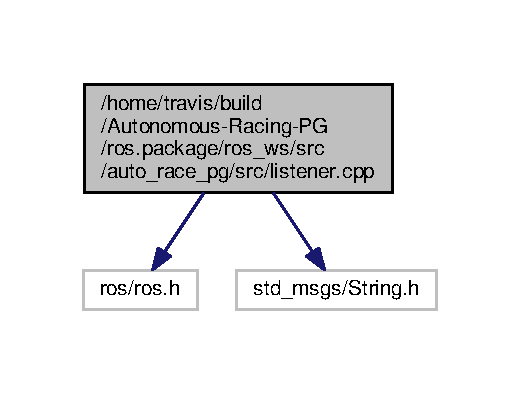
\includegraphics[width=250pt]{listener_8cpp__incl}
\end{center}
\end{figure}
\subsection*{Functions}
\begin{DoxyCompactItemize}
\item 
void \hyperlink{listener_8cpp_ae5c0c11b4a60030ee8df1a3ae0b6f758}{chatter\+Callback} (const std\+\_\+msgs\+::\+String\+::\+Const\+Ptr \&msg)
\item 
int \hyperlink{listener_8cpp_a3c04138a5bfe5d72780bb7e82a18e627}{main} (int argc, char $\ast$$\ast$argv)
\end{DoxyCompactItemize}


\subsection{Function Documentation}
\index{listener.\+cpp@{listener.\+cpp}!chatter\+Callback@{chatter\+Callback}}
\index{chatter\+Callback@{chatter\+Callback}!listener.\+cpp@{listener.\+cpp}}
\subsubsection[{\texorpdfstring{chatter\+Callback(const std\+\_\+msgs\+::\+String\+::\+Const\+Ptr \&msg)}{chatterCallback(const std_msgs::String::ConstPtr &msg)}}]{\setlength{\rightskip}{0pt plus 5cm}void chatter\+Callback (
\begin{DoxyParamCaption}
\item[{const std\+\_\+msgs\+::\+String\+::\+Const\+Ptr \&}]{msg}
\end{DoxyParamCaption}
)}\hypertarget{listener_8cpp_ae5c0c11b4a60030ee8df1a3ae0b6f758}{}\label{listener_8cpp_ae5c0c11b4a60030ee8df1a3ae0b6f758}


Definition at line 5 of file listener.\+cpp.



Here is the caller graph for this function\+:
\nopagebreak
\begin{figure}[H]
\begin{center}
\leavevmode
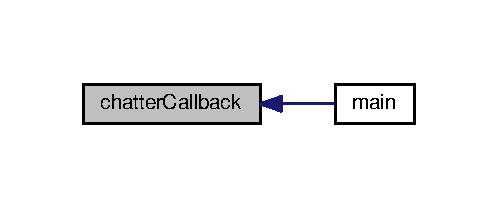
\includegraphics[width=239pt]{listener_8cpp_ae5c0c11b4a60030ee8df1a3ae0b6f758_icgraph}
\end{center}
\end{figure}


\index{listener.\+cpp@{listener.\+cpp}!main@{main}}
\index{main@{main}!listener.\+cpp@{listener.\+cpp}}
\subsubsection[{\texorpdfstring{main(int argc, char $\ast$$\ast$argv)}{main(int argc, char **argv)}}]{\setlength{\rightskip}{0pt plus 5cm}int main (
\begin{DoxyParamCaption}
\item[{int}]{argc, }
\item[{char $\ast$$\ast$}]{argv}
\end{DoxyParamCaption}
)}\hypertarget{listener_8cpp_a3c04138a5bfe5d72780bb7e82a18e627}{}\label{listener_8cpp_a3c04138a5bfe5d72780bb7e82a18e627}


Definition at line 10 of file listener.\+cpp.



Here is the call graph for this function\+:
\nopagebreak
\begin{figure}[H]
\begin{center}
\leavevmode
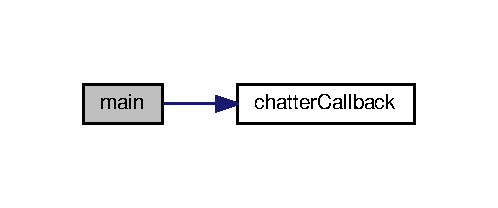
\includegraphics[width=239pt]{listener_8cpp_a3c04138a5bfe5d72780bb7e82a18e627_cgraph}
\end{center}
\end{figure}



\hypertarget{talker_8cpp}{}\section{/home/travis/build/\+Autonomous-\/\+Racing-\/\+P\+G/ros.package/docs/master/ros\+\_\+ws/src/auto\+\_\+race\+\_\+pg/src/talker.cpp File Reference}
\label{talker_8cpp}\index{/home/travis/build/\+Autonomous-\/\+Racing-\/\+P\+G/ros.\+package/docs/master/ros\+\_\+ws/src/auto\+\_\+race\+\_\+pg/src/talker.\+cpp@{/home/travis/build/\+Autonomous-\/\+Racing-\/\+P\+G/ros.\+package/docs/master/ros\+\_\+ws/src/auto\+\_\+race\+\_\+pg/src/talker.\+cpp}}
{\ttfamily \#include \char`\"{}ros/ros.\+h\char`\"{}}\\*
{\ttfamily \#include \char`\"{}std\+\_\+msgs/\+String.\+h\char`\"{}}\\*
{\ttfamily \#include $<$sstream$>$}\\*
Include dependency graph for talker.\+cpp\+:
\nopagebreak
\begin{figure}[H]
\begin{center}
\leavevmode
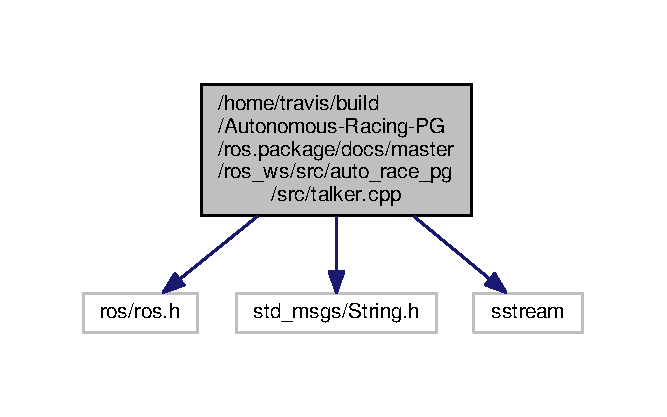
\includegraphics[width=320pt]{talker_8cpp__incl}
\end{center}
\end{figure}
\subsection*{Functions}
\begin{DoxyCompactItemize}
\item 
int \hyperlink{talker_8cpp_a3c04138a5bfe5d72780bb7e82a18e627}{main} (int argc, char $\ast$$\ast$argv)
\end{DoxyCompactItemize}


\subsection{Function Documentation}
\index{talker.\+cpp@{talker.\+cpp}!main@{main}}
\index{main@{main}!talker.\+cpp@{talker.\+cpp}}
\subsubsection[{\texorpdfstring{main(int argc, char $\ast$$\ast$argv)}{main(int argc, char **argv)}}]{\setlength{\rightskip}{0pt plus 5cm}int main (
\begin{DoxyParamCaption}
\item[{int}]{argc, }
\item[{char $\ast$$\ast$}]{argv}
\end{DoxyParamCaption}
)}\hypertarget{talker_8cpp_a3c04138a5bfe5d72780bb7e82a18e627}{}\label{talker_8cpp_a3c04138a5bfe5d72780bb7e82a18e627}


Definition at line 6 of file talker.\+cpp.


\hypertarget{test__auto__race__pg_8cpp}{}\section{/home/travis/build/\+Autonomous-\/\+Racing-\/\+P\+G/ros.package/ros\+\_\+ws/src/auto\+\_\+race\+\_\+pg/test/test\+\_\+auto\+\_\+race\+\_\+pg.cpp File Reference}
\label{test__auto__race__pg_8cpp}\index{/home/travis/build/\+Autonomous-\/\+Racing-\/\+P\+G/ros.\+package/ros\+\_\+ws/src/auto\+\_\+race\+\_\+pg/test/test\+\_\+auto\+\_\+race\+\_\+pg.\+cpp@{/home/travis/build/\+Autonomous-\/\+Racing-\/\+P\+G/ros.\+package/ros\+\_\+ws/src/auto\+\_\+race\+\_\+pg/test/test\+\_\+auto\+\_\+race\+\_\+pg.\+cpp}}
{\ttfamily \#include $<$cstdlib$>$}\\*
{\ttfamily \#include $<$gtest/gtest.\+h$>$}\\*
Include dependency graph for test\+\_\+auto\+\_\+race\+\_\+pg.\+cpp\+:
\nopagebreak
\begin{figure}[H]
\begin{center}
\leavevmode
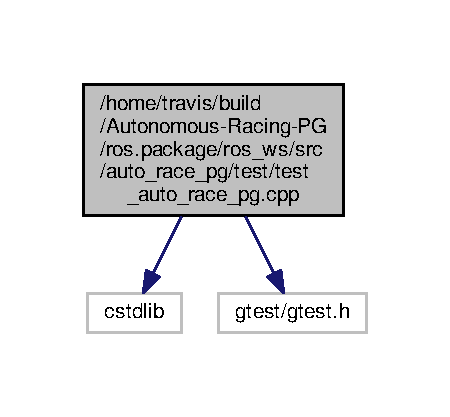
\includegraphics[width=216pt]{test__auto__race__pg_8cpp__incl}
\end{center}
\end{figure}
\subsection*{Functions}
\begin{DoxyCompactItemize}
\item 
\hyperlink{test__auto__race__pg_8cpp_abdd1a026bf2a8a181d4f4f61169c22f9}{T\+E\+ST} (dummy\+\_\+test, dummy\+\_\+test\+\_\+01)
\item 
\hyperlink{test__auto__race__pg_8cpp_a6accdba7cce21b4fbadc9847942eccee}{T\+E\+ST} (dummy\+\_\+test, dummy\+\_\+test\+\_\+02)
\item 
int \hyperlink{test__auto__race__pg_8cpp_a3c04138a5bfe5d72780bb7e82a18e627}{main} (int argc, char $\ast$$\ast$argv)
\end{DoxyCompactItemize}


\subsection{Function Documentation}
\index{test\+\_\+auto\+\_\+race\+\_\+pg.\+cpp@{test\+\_\+auto\+\_\+race\+\_\+pg.\+cpp}!main@{main}}
\index{main@{main}!test\+\_\+auto\+\_\+race\+\_\+pg.\+cpp@{test\+\_\+auto\+\_\+race\+\_\+pg.\+cpp}}
\subsubsection[{\texorpdfstring{main(int argc, char $\ast$$\ast$argv)}{main(int argc, char **argv)}}]{\setlength{\rightskip}{0pt plus 5cm}int main (
\begin{DoxyParamCaption}
\item[{int}]{argc, }
\item[{char $\ast$$\ast$}]{argv}
\end{DoxyParamCaption}
)}\hypertarget{test__auto__race__pg_8cpp_a3c04138a5bfe5d72780bb7e82a18e627}{}\label{test__auto__race__pg_8cpp_a3c04138a5bfe5d72780bb7e82a18e627}


Definition at line 20 of file test\+\_\+auto\+\_\+race\+\_\+pg.\+cpp.

\index{test\+\_\+auto\+\_\+race\+\_\+pg.\+cpp@{test\+\_\+auto\+\_\+race\+\_\+pg.\+cpp}!T\+E\+ST@{T\+E\+ST}}
\index{T\+E\+ST@{T\+E\+ST}!test\+\_\+auto\+\_\+race\+\_\+pg.\+cpp@{test\+\_\+auto\+\_\+race\+\_\+pg.\+cpp}}
\subsubsection[{\texorpdfstring{T\+E\+S\+T(dummy\+\_\+test, dummy\+\_\+test\+\_\+01)}{TEST(dummy_test, dummy_test_01)}}]{\setlength{\rightskip}{0pt plus 5cm}T\+E\+ST (
\begin{DoxyParamCaption}
\item[{dummy\+\_\+test}]{, }
\item[{dummy\+\_\+test\+\_\+01}]{}
\end{DoxyParamCaption}
)}\hypertarget{test__auto__race__pg_8cpp_abdd1a026bf2a8a181d4f4f61169c22f9}{}\label{test__auto__race__pg_8cpp_abdd1a026bf2a8a181d4f4f61169c22f9}


Definition at line 10 of file test\+\_\+auto\+\_\+race\+\_\+pg.\+cpp.

\index{test\+\_\+auto\+\_\+race\+\_\+pg.\+cpp@{test\+\_\+auto\+\_\+race\+\_\+pg.\+cpp}!T\+E\+ST@{T\+E\+ST}}
\index{T\+E\+ST@{T\+E\+ST}!test\+\_\+auto\+\_\+race\+\_\+pg.\+cpp@{test\+\_\+auto\+\_\+race\+\_\+pg.\+cpp}}
\subsubsection[{\texorpdfstring{T\+E\+S\+T(dummy\+\_\+test, dummy\+\_\+test\+\_\+02)}{TEST(dummy_test, dummy_test_02)}}]{\setlength{\rightskip}{0pt plus 5cm}T\+E\+ST (
\begin{DoxyParamCaption}
\item[{dummy\+\_\+test}]{, }
\item[{dummy\+\_\+test\+\_\+02}]{}
\end{DoxyParamCaption}
)}\hypertarget{test__auto__race__pg_8cpp_a6accdba7cce21b4fbadc9847942eccee}{}\label{test__auto__race__pg_8cpp_a6accdba7cce21b4fbadc9847942eccee}


Definition at line 15 of file test\+\_\+auto\+\_\+race\+\_\+pg.\+cpp.


%--- End generated contents ---

% Index
\backmatter
\newpage
\phantomsection
\clearemptydoublepage
\addcontentsline{toc}{chapter}{Index}
\printindex

\end{document}
